\documentclass[12pt]{article}\usepackage[]{graphicx}\usepackage[]{color}
% maxwidth is the original width if it is less than linewidth
% otherwise use linewidth (to make sure the graphics do not exceed the margin)
\makeatletter
\def\maxwidth{ %
  \ifdim\Gin@nat@width>\linewidth
    \linewidth
  \else
    \Gin@nat@width
  \fi
}
\makeatother

\definecolor{fgcolor}{rgb}{0.345, 0.345, 0.345}
\newcommand{\hlnum}[1]{\textcolor[rgb]{0.686,0.059,0.569}{#1}}%
\newcommand{\hlstr}[1]{\textcolor[rgb]{0.192,0.494,0.8}{#1}}%
\newcommand{\hlcom}[1]{\textcolor[rgb]{0.678,0.584,0.686}{\textit{#1}}}%
\newcommand{\hlopt}[1]{\textcolor[rgb]{0,0,0}{#1}}%
\newcommand{\hlstd}[1]{\textcolor[rgb]{0.345,0.345,0.345}{#1}}%
\newcommand{\hlkwa}[1]{\textcolor[rgb]{0.161,0.373,0.58}{\textbf{#1}}}%
\newcommand{\hlkwb}[1]{\textcolor[rgb]{0.69,0.353,0.396}{#1}}%
\newcommand{\hlkwc}[1]{\textcolor[rgb]{0.333,0.667,0.333}{#1}}%
\newcommand{\hlkwd}[1]{\textcolor[rgb]{0.737,0.353,0.396}{\textbf{#1}}}%
\let\hlipl\hlkwb

\usepackage{framed}
\makeatletter
\newenvironment{kframe}{%
 \def\at@end@of@kframe{}%
 \ifinner\ifhmode%
  \def\at@end@of@kframe{\end{minipage}}%
  \begin{minipage}{\columnwidth}%
 \fi\fi%
 \def\FrameCommand##1{\hskip\@totalleftmargin \hskip-\fboxsep
 \colorbox{shadecolor}{##1}\hskip-\fboxsep
     % There is no \\@totalrightmargin, so:
     \hskip-\linewidth \hskip-\@totalleftmargin \hskip\columnwidth}%
 \MakeFramed {\advance\hsize-\width
   \@totalleftmargin\z@ \linewidth\hsize
   \@setminipage}}%
 {\par\unskip\endMakeFramed%
 \at@end@of@kframe}
\makeatother

\definecolor{shadecolor}{rgb}{.97, .97, .97}
\definecolor{messagecolor}{rgb}{0, 0, 0}
\definecolor{warningcolor}{rgb}{1, 0, 1}
\definecolor{errorcolor}{rgb}{1, 0, 0}
\newenvironment{knitrout}{}{} % an empty environment to be redefined in TeX

\usepackage{alltt}

\usepackage{xr}

\makeatletter
\newcommand*{\addFileDependency}[1]{% argument=file name and extension
  \typeout{(#1)}
  \@addtofilelist{#1}
  \IfFileExists{#1}{}{\typeout{No file #1.}}
}
\makeatother

\newcommand*{\myexternaldocument}[1]{%
    \externaldocument{#1}%
    \addFileDependency{#1.tex}%
    \addFileDependency{#1.aux}%
}
\myexternaldocument{MainResults}

\usepackage{amsmath,amsfonts,amsthm,amssymb,thmtools}
\usepackage{bm}
\usepackage{natbib}
%\usepackage{fullpage}
\usepackage{graphicx}
\usepackage{float}
\usepackage{placeins}
%\usepackage{authblk}
\usepackage{comment}
\usepackage{tikz}
\usepackage{booktabs}
\usepackage{array}

\usetikzlibrary{calc}

%\pdfminorversion=4
% NOTE: To produce blinded version, replace "0" with "1" below.
\newcommand{\blind}{0}

\input{notation.tex}
\newcommand\independent{\protect\mathpalette{\protect\independenT}{\perp}}
\def\independenT#1#2{\mathrel{\rlap{$#1#2$}\mkern2mu{#1#2}}}
\DeclareMathOperator*{\argmin}{arg\,min}
\newtheorem{prop}{Proposition}


% DON'T change margins - should be 1 inch all around.
\addtolength{\oddsidemargin}{-.5in}%
\addtolength{\evensidemargin}{-.5in}%
\addtolength{\textwidth}{1in}%
\addtolength{\textheight}{.8in}%
\addtolength{\topmargin}{-.8in}%
\IfFileExists{upquote.sty}{\usepackage{upquote}}{}
\begin{document}

%\bibliographystyle{natbib}

\def\spacingset#1{\renewcommand{\baselinestretch}%
{#1}\small\normalsize} \spacingset{1}


%%%%%%%%%%%%%%%%%%%%%%%%%%%%%%%%%%%%%%%%%%%%%%%%%%%%%%%%%%%%%%%%%%%%%%%%%%%%%%

\if1\blind
{
  \title{\bf Replication Document for the Main Results in ``Precise Unbiased Estimation in Randomized Experiments using Auxiliary Observational Data''}
  \author{Johann A. Gagnon-Bartsch\thanks{This work was partially
      supported by IES grant R305D210031}\hspace{.2cm}\footnote{These authors contributed equally.}\\
    Department of Statistics, University of Michigan\\
    and \\
    Adam C. Sales${}^\dagger$\\
    Department of Mathematical Sciences, Worcester Polytechnic
    Institute\\
        and \\
    Edward Wu \\
    Department of Statistics, University of Michigan\\
    and \\
    Anthony F. Botelho \\
    Department of Computer Science, Worcester Polytechnic
    Institute\\
    and \\
    John A. Erickson \\
    Data Science Program, Worcester Polytechnic
    Institute\\
    and \\
    Neil T. Heffernan \\
    Department of Computer Science, Worcester Polytechnic
    Institute\\
    and \\
    Luke W. Miratrix \\
    Graduate School of Education, Harvard University




  }
  \date{}
  \maketitle
} \fi

\if0\blind
{
  \bigskip
  \bigskip
  \bigskip
  \begin{center}
    \LARGE\bf Replication Document for the Main Results in ``Precise Unbiased Estimation in Randomized Experiments using Auxiliary Observational Data''
\end{center}
  \medskip
} \fi

\section{Preliminaries}

This document will reproduce all of the tables and figures from the
manuscript. The tables and figures will appear in the compiled version
of this PDF, as well as in stand-alone files to be incorporated into
the main manuscript.

\begin{knitrout}
\definecolor{shadecolor}{rgb}{0.969, 0.969, 0.969}\color{fgcolor}\begin{kframe}
\begin{alltt}
\hlstd{opts_chunk}\hlopt{$}\hlkwd{set}\hlstd{(}\hlkwc{message}\hlstd{=}\hlnum{FALSE}\hlstd{,}\hlkwc{warning}\hlstd{=}\hlnum{FALSE}\hlstd{,}\hlkwc{error}\hlstd{=}\hlnum{FALSE}\hlstd{,}\hlkwc{echo}\hlstd{=}\hlnum{TRUE}\hlstd{,}\hlkwc{cache}\hlstd{=}\hlnum{TRUE}\hlstd{,}\hlkwc{dev}\hlstd{=}\hlstr{'tikz'}\hlstd{)}
\end{alltt}
\end{kframe}
\end{knitrout}

\begin{knitrout}
\definecolor{shadecolor}{rgb}{0.969, 0.969, 0.969}\color{fgcolor}\begin{kframe}
\begin{alltt}
\hlkwd{library}\hlstd{(scales)}
\hlkwd{library}\hlstd{(tidyverse)}
\hlkwd{library}\hlstd{(loop.estimator)}
\hlkwd{library}\hlstd{(kableExtra)}
\hlkwd{library}\hlstd{(xtable)}
\hlkwd{library}\hlstd{(knitr)}
\hlkwd{library}\hlstd{(tikzDevice)}




\hlcom{## specialized versions of the LOOP estimator}
\hlkwd{source}\hlstd{(}\hlstr{'code/loop_ols.R'}\hlstd{)}
\hlkwd{source}\hlstd{(}\hlstr{'code/loop_ext.R'}\hlstd{)}
\hlcom{## functions for estimating effects}
\hlkwd{source}\hlstd{(}\hlstr{'code/analysisFunctions.r'}\hlstd{)}
\end{alltt}
\end{kframe}
\end{knitrout}

Names of covariates for within-sample covariate adjustment:
\begin{knitrout}
\definecolor{shadecolor}{rgb}{0.969, 0.969, 0.969}\color{fgcolor}\begin{kframe}
\begin{alltt}
\hlstd{covNames} \hlkwb{<-} \hlkwd{c}\hlstd{(}
    \hlstr{"Prior.Problem.Count"}\hlstd{,}
    \hlstr{"Prior.Percent.Correct"}\hlstd{,}
    \hlstr{"Prior.Assignments.Assigned"}\hlstd{,}
    \hlstr{"Prior.Percent.Completion"}\hlstd{,}
    \hlstr{"Prior.Class.Percent.Completion"}\hlstd{,}
    \hlstr{"Prior.Homework.Assigned"}\hlstd{,}
    \hlstr{"Prior.Homework.Percent.Completion"}\hlstd{,}
    \hlstr{"Prior.Class.Homework.Percent.Completion"}\hlstd{,}
    \hlstr{"male"}\hlstd{,}
    \hlstr{"unknownGender"}\hlstd{)}\hlcom{#)}
\end{alltt}
\end{kframe}
\end{knitrout}

\section{Data}

Here we load in the data for estimating effects and standard errors
using several different methods discussed in the manuscript.
Note that the predictions from the model fit in the remnant are
already part of the datasets (which are themselves part of the GitHub
repository) under the column name \texttt{p\_complete}.

Load in and clean the data:\\

\begin{knitrout}
\definecolor{shadecolor}{rgb}{0.969, 0.969, 0.969}\color{fgcolor}\begin{kframe}
\begin{alltt}
\hlkwd{source}\hlstd{(}\hlstr{'code/dataPrep.r'}\hlstd{)}
\end{alltt}
\end{kframe}
\end{knitrout}

Replicating Table \ref{tab:covariates} from the manuscript:

\begin{kframe}
\begin{alltt}
\hlkwd{source}\hlstd{(}\hlstr{'code/covTable.r'}\hlstd{)}
\hlkwd{print}\hlstd{(covTable,} \hlkwc{add.to.row}\hlstd{=ATR)}
\end{alltt}
\end{kframe}% latex table generated in R 4.0.3 by xtable 1.8-4 package
% Fri May 21 13:03:33 2021
\begin{table}[ht]
\centering
\begin{tabular}{rrrr}
  \hline
 & Mean & SD & \% Missing \\ 
  \hline
Problem Count & 603.11 & 784.29 & 2 \\ 
  Percent Correct & 0.68 & 0.13 & 2 \\ 
  Assignments Assigned & 103.92 & 412.15 & 13 \\ 
  Percent Completion & 0.89 & 0.21 & 13 \\ 
  Class Percent Completion & 0.90 & 0.13 & 22 \\ 
  Homework Assigned & 25.82 & 29.87 & 50 \\ 
  Homework Percent Completion & 0.93 & 0.16 & 59 \\ 
  Class Homework Percent Completion & 0.93 & 0.09 & 56 \\ 
   Guessed Gender&Male: 36\%&Female: 36\%&Unknown: 28\%\\
 \hline
\end{tabular}
\caption{Pooled summary statistics for aggregate prior ASSISTments performance used as within-sample covariates.} 
\label{tab:covariates}
\end{table}


\subsection{Imputing Missing Covariates}

To impute missing covariate values, when possible we imputed the
classroom mean covariate value for students working on that skill
builder.
When there were no other available values for a covariate for students
in the same classroom working on the same skill builder, we imputed
with the global mean of students working on that skill builder.
Since covariates are all pre-treatment and the imputation did not
depend on treatment status, the imputed covariates are themselves
covariates, measured for all subjects.
Therefore, we need not correct for the imputation scheme in our
treatment effect estimation.

\begin{knitrout}
\definecolor{shadecolor}{rgb}{0.969, 0.969, 0.969}\color{fgcolor}\begin{kframe}
\begin{alltt}
\hlcom{### first fill in with class/problem_set mean}
\hlcom{### if that doesn't work, fill in with problem_set mean}
\hlstd{dat} \hlkwb{<-} \hlstd{dat}\hlopt
    \hlkwd{group_by}\hlstd{(Class.ID,problem_set)}\hlopt
    \hlkwd{mutate}\hlstd{(}\hlkwd{across}\hlstd{(}\hlkwd{all_of}\hlstd{(covNames),}\hlopt{~}\hlkwd{ifelse}\hlstd{(}\hlkwd{is.finite}\hlstd{(.),.,}\hlkwd{mean}\hlstd{(.,}\hlkwc{na.rm}\hlstd{=}\hlnum{TRUE}\hlstd{))))}\hlopt
    \hlkwd{group_by}\hlstd{(problem_set)}\hlopt
    \hlkwd{mutate}\hlstd{(}\hlkwd{across}\hlstd{(}\hlkwd{all_of}\hlstd{(covNames),}\hlopt{~}\hlkwd{ifelse}\hlstd{(}\hlkwd{is.finite}\hlstd{(.),.,}\hlkwd{mean}\hlstd{(.,}\hlkwc{na.rm}\hlstd{=}\hlnum{TRUE}\hlstd{))))}\hlopt
    \hlkwd{ungroup}\hlstd{()}

\hlkwd{stopifnot}\hlstd{(}\hlkwd{all}\hlstd{(}\hlkwd{sapply}\hlstd{(covNames,}\hlkwa{function}\hlstd{(}\hlkwc{x}\hlstd{)} \hlkwd{mean}\hlstd{(}\hlkwd{is.finite}\hlstd{(dat[[x]])))}\hlopt{==}\hlnum{1}\hlstd{))}
\end{alltt}
\end{kframe}
\end{knitrout}





\section{Estimate Effects}

Here we estimate effects of treatment for each of the
33 skill builders in the dataset.
The functions for estimating effects are all found in the file
\texttt{code/analysisFunctions.r}.
This includes the function \texttt{full()} which estimates all five
treatment effects discussed in the paper.

\begin{knitrout}
\definecolor{shadecolor}{rgb}{0.969, 0.969, 0.969}\color{fgcolor}\begin{kframe}
\begin{alltt}
\hlstd{fullres} \hlkwb{<-} \hlkwd{sapply}\hlstd{(}\hlkwd{levels}\hlstd{(dat}\hlopt{$}\hlstd{problem_set),full,}\hlkwc{dat}\hlstd{=dat,}\hlkwc{covNames}\hlstd{=covNames,}\hlkwc{simplify}\hlstd{=}\hlnum{FALSE}\hlstd{)}

\hlcom{### name the problem sets based on the SE from the simple difference estimator}
\hlstd{rnk} \hlkwb{<-} \hlkwd{rank}\hlstd{(}\hlkwd{sapply}\hlstd{(fullres,}\hlkwa{function}\hlstd{(}\hlkwc{x}\hlstd{) x[}\hlstr{'simpDiff'}\hlstd{,}\hlstr{'se'}\hlstd{]))}
\hlkwd{names}\hlstd{(fullres)} \hlkwb{<-} \hlkwd{as.character}\hlstd{(rnk)}

\hlkwa{for}\hlstd{(i} \hlkwa{in} \hlnum{1}\hlopt{:}\hlkwd{length}\hlstd{(fullres))}
    \hlkwd{attr}\hlstd{(fullres[[i]],}\hlstr{'psid'}\hlstd{)} \hlkwb{<-} \hlkwd{levels}\hlstd{(dat}\hlopt{$}\hlstd{problem_set)[i]}

\hlkwd{save}\hlstd{(fullres,}\hlkwc{file}\hlstd{=}\hlstr{'results/fullres.RData'}\hlstd{)}

\hlstd{dat}\hlopt{$}\hlstd{ps} \hlkwb{<-} \hlstd{rnk[}\hlkwd{as.character}\hlstd{(dat}\hlopt{$}\hlstd{problem_set)]}
\end{alltt}
\end{kframe}
\end{knitrout}

Replicate Table \ref{tab:info} (Now in an appendix, I think).
The numbering of the experiments derives from the estimated standard
errors, so this comes after effect estimation.
\begin{kframe}
\begin{alltt}
\hlkwd{source}\hlstd{(}\hlstr{'code/psTable.r'}\hlstd{)}

 \hlkwd{kbl}\hlstd{(tab,}

           \hlkwc{booktabs}\hlstd{=}\hlnum{FALSE}\hlstd{,}
           \hlkwc{col.names}\hlstd{=}\hlkwd{rep}\hlstd{(}\hlkwd{c}\hlstd{(}\hlstr{""}\hlstd{,}\hlkwd{rep}\hlstd{(}\hlkwd{c}\hlstd{(}\hlstr{"Trt"}\hlstd{,}\hlstr{"Ctl"}\hlstd{),}\hlnum{2}\hlstd{)),}\hlnum{2}\hlstd{),}
           \hlkwc{caption}\hlstd{=}\hlstr{"Sample sizes and \textbackslash{}\textbackslash{}% homework completion by treatment group in each of the 33 A/B tests."}\hlstd{,}
           \hlkwc{label}\hlstd{=}\hlstr{"info"}\hlstd{)}\hlopt
    \hlkwd{kable_styling}\hlstd{()}\hlopt
    \hlkwd{column_spec}\hlstd{(}\hlnum{5}\hlstd{,}\hlkwc{border_right}\hlstd{=}\hlnum{TRUE}\hlstd{)}\hlopt
    \hlkwd{add_header_above}\hlstd{(}\hlkwd{rep}\hlstd{(}\hlkwd{c}\hlstd{(}\hlstr{"Experiment"}\hlstd{=}\hlnum{1}\hlstd{,}\hlstr{"n"}\hlstd{=}\hlnum{2}\hlstd{,}\hlstr{"% Complete"}\hlstd{=}\hlnum{2}\hlstd{),}\hlnum{2}\hlstd{))}
\end{alltt}
\end{kframe}\begin{table}

\caption{\label{tab:info}Sample sizes and \% homework completion by treatment group in each of the 33 A/B tests.}
\centering
\begin{tabular}[t]{r|r|r|r|>{}r||r|r|r|r|r}
\hline
\multicolumn{1}{c|}{Experiment} & \multicolumn{2}{c|}{n} & \multicolumn{2}{c|}{\% Complete} & \multicolumn{1}{c|}{Experiment} & \multicolumn{2}{c|}{n} & \multicolumn{2}{c}{\% Complete} \\
\cline{1-1} \cline{2-3} \cline{4-5} \cline{6-6} \cline{7-8} \cline{9-10}
 & Trt & Ctl & Trt & Ctl &  & Trt & Ctl & Trt & Ctl\\
\hline
1 & 956 & 961 & 93 & 93 & 18 & 188 & 193 & 89 & 85\\
\hline
2 & 330 & 365 & 98 & 96 & 19 & 199 & 213 & 89 & 82\\
\hline
3 & 680 & 650 & 86 & 88 & 20 & 264 & 281 & 81 & 79\\
\hline
4 & 943 & 921 & 70 & 68 & 21 & 242 & 266 & 81 & 76\\
\hline
5 & 931 & 900 & 61 & 64 & 22 & 215 & 211 & 82 & 82\\
\hline
6 & 355 & 349 & 88 & 88 & 23 & 281 & 234 & 73 & 69\\
\hline
7 & 492 & 463 & 79 & 81 & 24 & 269 & 288 & 65 & 59\\
\hline
8 & 231 & 197 & 92 & 91 & 25 & 224 & 233 & 73 & 74\\
\hline
9 & 367 & 387 & 83 & 82 & 26 & 270 & 253 & 63 & 61\\
\hline
10 & 617 & 587 & 67 & 62 & 27 & 228 & 244 & 68 & 64\\
\hline
11 & 338 & 289 & 88 & 84 & 28 & 201 & 228 & 73 & 69\\
\hline
12 & 478 & 476 & 76 & 73 & 29 & 238 & 259 & 44 & 54\\
\hline
13 & 193 & 209 & 93 & 89 & 30 & 74 & 92 & 91 & 84\\
\hline
14 & 404 & 451 & 73 & 69 & 31 & 69 & 67 & 91 & 87\\
\hline
15 & 265 & 275 & 85 & 84 & 32 & 76 & 81 & 62 & 70\\
\hline
16 & 165 & 170 & 92 & 89 & 33 & 15 & 11 & 73 & 55\\
\hline
17 & 259 & 246 & 82 & 85 & NA & NA & NA & NA & NA\\
\hline
\end{tabular}
\end{table}




\section{Figures}

The following code creates a dataset called \texttt{comparisons} that
includes the sampling variance ratios comparing each method to the
others, for each problem set.
It also produces a table (which is not in the manuscript) giving the estimated standard error for each method and each
experiment.
\begin{kframe}
\begin{alltt}
\hlkwd{source}\hlstd{(}\hlstr{'code/figurePrep.r'}\hlstd{)}

\hlstd{pwidePrint} \hlkwb{<-} \hlstd{pwide}
\hlkwd{names}\hlstd{(pwidePrint)[}\hlopt{-}\hlnum{1}\hlstd{]} \hlkwb{<-} \hlkwd{paste0}\hlstd{(}\hlstr{'$'}\hlstd{,methodName[}\hlkwd{names}\hlstd{(pwidePrint)[}\hlopt{-}\hlnum{1}\hlstd{]],}\hlstr{'$'}\hlstd{)}
\hlkwd{kable}\hlstd{(pwidePrint,}\hlkwc{row.names}\hlstd{=}\hlnum{FALSE}\hlstd{,}\hlkwc{caption}\hlstd{=}\hlstr{"Estimated standard error for the ATE in each skill builder, using each method discussed in the manuscript"}\hlstd{,}\hlkwc{label}\hlstd{=}\hlstr{"tab:SEs"}\hlstd{,}\hlkwc{digits}\hlstd{=}\hlnum{3}\hlstd{,}\hlkwc{escape}\hlstd{=}\hlnum{FALSE}\hlstd{)}
\end{alltt}
\end{kframe}\begin{table}

\caption{\label{tab:tab:SEs}Estimated standard error for the ATE in each skill builder, using each method discussed in the manuscript}
\centering
\begin{tabular}[t]{l|r|r|r|r|r}
\hline
experiment & $\trcpen$ & $\trc$ & $\tss[\bx,\mathrm{RF}]$ & $\trebar$ & $\tsd$\\
\hline
1 & 0.010 & 0.011 & 0.011 & 0.011 & 0.012\\
\hline
10 & 0.021 & 0.024 & 0.021 & 0.024 & 0.028\\
\hline
11 & 0.026 & 0.027 & 0.026 & 0.028 & 0.028\\
\hline
12 & 0.022 & 0.026 & 0.022 & 0.026 & 0.028\\
\hline
13 & 0.029 & 0.029 & 0.030 & 0.032 & 0.029\\
\hline
14 & 0.029 & 0.029 & 0.030 & 0.029 & 0.031\\
\hline
15 & 0.028 & 0.029 & 0.029 & 0.029 & 0.031\\
\hline
16 & 0.031 & 0.031 & 0.031 & 0.031 & 0.032\\
\hline
17 & 0.031 & 0.032 & 0.031 & 0.032 & 0.033\\
\hline
18 & 0.032 & 0.032 & 0.033 & 0.033 & 0.034\\
\hline
19 & 0.035 & 0.034 & 0.037 & 0.038 & 0.034\\
\hline
2 & 0.013 & 0.012 & 0.013 & 0.017 & 0.013\\
\hline
20 & 0.032 & 0.033 & 0.033 & 0.034 & 0.034\\
\hline
21 & 0.034 & 0.034 & 0.035 & 0.034 & 0.036\\
\hline
22 & 0.035 & 0.036 & 0.034 & 0.036 & 0.037\\
\hline
23 & 0.034 & 0.037 & 0.035 & 0.038 & 0.040\\
\hline
24 & 0.030 & 0.040 & 0.029 & 0.041 & 0.041\\
\hline
25 & 0.038 & 0.040 & 0.038 & 0.040 & 0.041\\
\hline
26 & 0.030 & 0.034 & 0.030 & 0.035 & 0.042\\
\hline
27 & 0.038 & 0.040 & 0.038 & 0.040 & 0.044\\
\hline
28 & 0.043 & 0.044 & 0.043 & 0.046 & 0.044\\
\hline
29 & 0.045 & 0.045 & 0.047 & 0.047 & 0.045\\
\hline
3 & 0.016 & 0.018 & 0.016 & 0.018 & 0.018\\
\hline
30 & 0.050 & 0.050 & 0.054 & 0.050 & 0.052\\
\hline
31 & 0.050 & 0.049 & 0.050 & 0.051 & 0.054\\
\hline
32 & 0.063 & 0.067 & 0.060 & 0.066 & 0.076\\
\hline
33 & 0.122 & 0.131 & 0.153 & 0.142 & 0.197\\
\hline
4 & 0.018 & 0.019 & 0.017 & 0.020 & 0.021\\
\hline
5 & 0.019 & 0.019 & 0.019 & 0.019 & 0.023\\
\hline
6 & 0.020 & 0.022 & 0.019 & 0.021 & 0.025\\
\hline
7 & 0.019 & 0.022 & 0.019 & 0.022 & 0.026\\
\hline
8 & 0.026 & 0.026 & 0.028 & 0.027 & 0.027\\
\hline
9 & 0.025 & 0.027 & 0.025 & 0.028 & 0.027\\
\hline
\end{tabular}
\end{table}



Figure \ref{fig:ses1}, comparing
$\tsd$,
$\trebar$, and $\trc$:

\begin{knitrout}
\definecolor{shadecolor}{rgb}{0.969, 0.969, 0.969}\color{fgcolor}\begin{kframe}
\begin{alltt}
\hlstd{p} \hlkwb{<-} \hlstd{comparisons}\hlopt
    \hlkwd{filter}\hlstd{(method1}\hlopt\hlkwd{c}\hlstd{(}\hlstr{'ReLOOP'}\hlstd{,}\hlstr{'Rebar'}\hlstd{),method2}\hlopt\hlkwd{c}\hlstd{(}\hlstr{'ReLOOPEN'}\hlstd{,}\hlstr{'Rebar'}\hlstd{,}\hlstr{'SimpleDifference'}\hlstd{))}\hlopt
    \hlkwd{ggplot}\hlstd{(}\hlkwd{aes}\hlstd{(ssMult))}\hlopt{+}\hlcom{#,fill=exGroup))+}
    \hlkwd{geom_dotplot}\hlstd{(} \hlkwc{method}\hlstd{=}\hlstr{"histodot"}\hlstd{,} \hlkwc{binwidth} \hlstd{=} \hlnum{.05} \hlstd{)}  \hlopt{+}
    \hlkwd{labs}\hlstd{(} \hlkwc{x} \hlstd{=} \hlstr{"Relative Ratio of Sample Variances"}\hlstd{,} \hlkwc{y}\hlstd{=}\hlstr{""} \hlstd{)} \hlopt{+}
    \hlkwd{geom_vline}\hlstd{(} \hlkwc{xintercept} \hlstd{=} \hlnum{1}\hlstd{,} \hlkwc{col}\hlstd{=}\hlstr{"red"} \hlstd{)} \hlopt{+}
    \hlkwd{facet_wrap}\hlstd{(}\hlopt{~}\hlstd{comp,}\hlkwc{nrow}\hlstd{=}\hlnum{1}\hlstd{)}\hlopt{+}
    \hlkwd{theme}\hlstd{(}\hlkwc{legend.position} \hlstd{=} \hlstr{"none"}\hlstd{,}
        \hlkwc{panel.grid} \hlstd{=} \hlkwd{element_blank}\hlstd{(),}
        \hlkwc{axis.title.y} \hlstd{=} \hlkwd{element_blank}\hlstd{(),}
        \hlkwc{axis.text.y}\hlstd{=} \hlkwd{element_blank}\hlstd{(),}
        \hlkwc{axis.ticks.y} \hlstd{=} \hlkwd{element_blank}\hlstd{(),}
        \hlkwc{text}\hlstd{=}\hlkwd{element_text}\hlstd{(}\hlkwc{size}\hlstd{=}\hlnum{12}\hlstd{),}
        \hlkwc{strip.text}\hlstd{=}\hlkwd{element_text}\hlstd{(}\hlkwc{size}\hlstd{=}\hlnum{12}\hlstd{,}\hlkwc{lineheight}\hlstd{=}\hlnum{0.5}\hlstd{))}

\hlkwd{tikz}\hlstd{(}\hlstr{'figure/fig4.tex'}\hlstd{,}\hlkwc{width}\hlstd{=}\hlnum{6.4}\hlstd{,}\hlkwc{height}\hlstd{=}\hlnum{2}\hlstd{,}\hlkwc{standAlone}\hlstd{=}\hlnum{FALSE}\hlstd{)}
\hlkwd{print}\hlstd{(p)}
\hlkwd{dev.off}\hlstd{()}
\end{alltt}
\begin{verbatim}
## tikz output 
##           2
\end{verbatim}
\end{kframe}
\end{knitrout}

\begin{figure}
\centering
% Created by tikzDevice version 0.12.3.1 on 2021-05-20 17:57:48
% !TEX encoding = UTF-8 Unicode
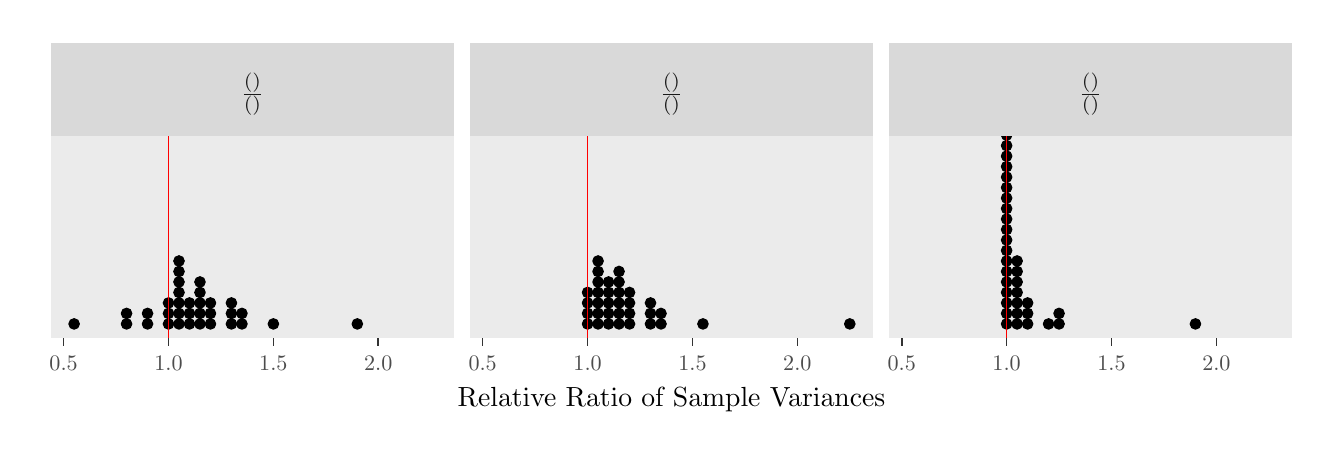
\begin{tikzpicture}[x=1pt,y=1pt]
\definecolor{fillColor}{RGB}{255,255,255}
\path[use as bounding box,fill=fillColor,fill opacity=0.00] (0,0) rectangle (462.53,144.54);
\begin{scope}
\path[clip] (  0.00,  0.00) rectangle (462.53,144.54);
\definecolor{drawColor}{RGB}{255,255,255}
\definecolor{fillColor}{RGB}{255,255,255}

\path[draw=drawColor,line width= 0.6pt,line join=round,line cap=round,fill=fillColor] (  0.00,  0.00) rectangle (462.53,144.54);
\end{scope}
\begin{scope}
\path[clip] (  8.25, 32.28) rectangle (154.18,105.24);
\definecolor{fillColor}{gray}{0.92}

\path[fill=fillColor] (  8.25, 32.28) rectangle (154.18,105.24);
\definecolor{drawColor}{RGB}{0,0,0}
\definecolor{fillColor}{RGB}{0,0,0}

\path[draw=drawColor,line width= 0.4pt,line join=round,line cap=round,fill=fillColor] ( 16.78, 37.49) circle (  1.90);

\path[draw=drawColor,line width= 0.4pt,line join=round,line cap=round,fill=fillColor] ( 35.73, 37.49) circle (  1.90);

\path[draw=drawColor,line width= 0.4pt,line join=round,line cap=round,fill=fillColor] ( 35.73, 41.28) circle (  1.90);

\path[draw=drawColor,line width= 0.4pt,line join=round,line cap=round,fill=fillColor] ( 43.31, 37.49) circle (  1.90);

\path[draw=drawColor,line width= 0.4pt,line join=round,line cap=round,fill=fillColor] ( 43.31, 41.28) circle (  1.90);

\path[draw=drawColor,line width= 0.4pt,line join=round,line cap=round,fill=fillColor] ( 50.89, 37.49) circle (  1.90);

\path[draw=drawColor,line width= 0.4pt,line join=round,line cap=round,fill=fillColor] ( 50.89, 41.28) circle (  1.90);

\path[draw=drawColor,line width= 0.4pt,line join=round,line cap=round,fill=fillColor] ( 50.89, 45.07) circle (  1.90);

\path[draw=drawColor,line width= 0.4pt,line join=round,line cap=round,fill=fillColor] ( 54.68, 37.49) circle (  1.90);

\path[draw=drawColor,line width= 0.4pt,line join=round,line cap=round,fill=fillColor] ( 54.68, 41.28) circle (  1.90);

\path[draw=drawColor,line width= 0.4pt,line join=round,line cap=round,fill=fillColor] ( 54.68, 45.07) circle (  1.90);

\path[draw=drawColor,line width= 0.4pt,line join=round,line cap=round,fill=fillColor] ( 54.68, 48.86) circle (  1.90);

\path[draw=drawColor,line width= 0.4pt,line join=round,line cap=round,fill=fillColor] ( 54.68, 52.65) circle (  1.90);

\path[draw=drawColor,line width= 0.4pt,line join=round,line cap=round,fill=fillColor] ( 54.68, 56.44) circle (  1.90);

\path[draw=drawColor,line width= 0.4pt,line join=round,line cap=round,fill=fillColor] ( 54.68, 60.23) circle (  1.90);

\path[draw=drawColor,line width= 0.4pt,line join=round,line cap=round,fill=fillColor] ( 58.47, 37.49) circle (  1.90);

\path[draw=drawColor,line width= 0.4pt,line join=round,line cap=round,fill=fillColor] ( 58.47, 41.28) circle (  1.90);

\path[draw=drawColor,line width= 0.4pt,line join=round,line cap=round,fill=fillColor] ( 58.47, 45.07) circle (  1.90);

\path[draw=drawColor,line width= 0.4pt,line join=round,line cap=round,fill=fillColor] ( 62.26, 37.49) circle (  1.90);

\path[draw=drawColor,line width= 0.4pt,line join=round,line cap=round,fill=fillColor] ( 62.26, 41.28) circle (  1.90);

\path[draw=drawColor,line width= 0.4pt,line join=round,line cap=round,fill=fillColor] ( 62.26, 45.07) circle (  1.90);

\path[draw=drawColor,line width= 0.4pt,line join=round,line cap=round,fill=fillColor] ( 62.26, 48.86) circle (  1.90);

\path[draw=drawColor,line width= 0.4pt,line join=round,line cap=round,fill=fillColor] ( 62.26, 52.65) circle (  1.90);

\path[draw=drawColor,line width= 0.4pt,line join=round,line cap=round,fill=fillColor] ( 66.05, 37.49) circle (  1.90);

\path[draw=drawColor,line width= 0.4pt,line join=round,line cap=round,fill=fillColor] ( 66.05, 41.28) circle (  1.90);

\path[draw=drawColor,line width= 0.4pt,line join=round,line cap=round,fill=fillColor] ( 66.05, 45.07) circle (  1.90);

\path[draw=drawColor,line width= 0.4pt,line join=round,line cap=round,fill=fillColor] ( 73.63, 37.49) circle (  1.90);

\path[draw=drawColor,line width= 0.4pt,line join=round,line cap=round,fill=fillColor] ( 73.63, 41.28) circle (  1.90);

\path[draw=drawColor,line width= 0.4pt,line join=round,line cap=round,fill=fillColor] ( 73.63, 45.07) circle (  1.90);

\path[draw=drawColor,line width= 0.4pt,line join=round,line cap=round,fill=fillColor] ( 77.42, 37.49) circle (  1.90);

\path[draw=drawColor,line width= 0.4pt,line join=round,line cap=round,fill=fillColor] ( 77.42, 41.28) circle (  1.90);

\path[draw=drawColor,line width= 0.4pt,line join=round,line cap=round,fill=fillColor] ( 88.79, 37.49) circle (  1.90);

\path[draw=drawColor,line width= 0.4pt,line join=round,line cap=round,fill=fillColor] (119.12, 37.49) circle (  1.90);
\definecolor{drawColor}{RGB}{255,0,0}

\path[draw=drawColor,line width= 0.6pt,line join=round] ( 50.89, 32.28) -- ( 50.89,105.24);
\end{scope}
\begin{scope}
\path[clip] (159.68, 32.28) rectangle (305.60,105.24);
\definecolor{fillColor}{gray}{0.92}

\path[fill=fillColor] (159.68, 32.28) rectangle (305.60,105.24);
\definecolor{drawColor}{RGB}{0,0,0}
\definecolor{fillColor}{RGB}{0,0,0}

\path[draw=drawColor,line width= 0.4pt,line join=round,line cap=round,fill=fillColor] (202.32, 37.49) circle (  1.90);

\path[draw=drawColor,line width= 0.4pt,line join=round,line cap=round,fill=fillColor] (202.32, 41.28) circle (  1.90);

\path[draw=drawColor,line width= 0.4pt,line join=round,line cap=round,fill=fillColor] (202.32, 45.07) circle (  1.90);

\path[draw=drawColor,line width= 0.4pt,line join=round,line cap=round,fill=fillColor] (202.32, 48.86) circle (  1.90);

\path[draw=drawColor,line width= 0.4pt,line join=round,line cap=round,fill=fillColor] (206.11, 37.49) circle (  1.90);

\path[draw=drawColor,line width= 0.4pt,line join=round,line cap=round,fill=fillColor] (206.11, 41.28) circle (  1.90);

\path[draw=drawColor,line width= 0.4pt,line join=round,line cap=round,fill=fillColor] (206.11, 45.07) circle (  1.90);

\path[draw=drawColor,line width= 0.4pt,line join=round,line cap=round,fill=fillColor] (206.11, 48.86) circle (  1.90);

\path[draw=drawColor,line width= 0.4pt,line join=round,line cap=round,fill=fillColor] (206.11, 52.65) circle (  1.90);

\path[draw=drawColor,line width= 0.4pt,line join=round,line cap=round,fill=fillColor] (206.11, 56.44) circle (  1.90);

\path[draw=drawColor,line width= 0.4pt,line join=round,line cap=round,fill=fillColor] (206.11, 60.23) circle (  1.90);

\path[draw=drawColor,line width= 0.4pt,line join=round,line cap=round,fill=fillColor] (209.90, 37.49) circle (  1.90);

\path[draw=drawColor,line width= 0.4pt,line join=round,line cap=round,fill=fillColor] (209.90, 41.28) circle (  1.90);

\path[draw=drawColor,line width= 0.4pt,line join=round,line cap=round,fill=fillColor] (209.90, 45.07) circle (  1.90);

\path[draw=drawColor,line width= 0.4pt,line join=round,line cap=round,fill=fillColor] (209.90, 48.86) circle (  1.90);

\path[draw=drawColor,line width= 0.4pt,line join=round,line cap=round,fill=fillColor] (209.90, 52.65) circle (  1.90);

\path[draw=drawColor,line width= 0.4pt,line join=round,line cap=round,fill=fillColor] (213.69, 37.49) circle (  1.90);

\path[draw=drawColor,line width= 0.4pt,line join=round,line cap=round,fill=fillColor] (213.69, 41.28) circle (  1.90);

\path[draw=drawColor,line width= 0.4pt,line join=round,line cap=round,fill=fillColor] (213.69, 45.07) circle (  1.90);

\path[draw=drawColor,line width= 0.4pt,line join=round,line cap=round,fill=fillColor] (213.69, 48.86) circle (  1.90);

\path[draw=drawColor,line width= 0.4pt,line join=round,line cap=round,fill=fillColor] (213.69, 52.65) circle (  1.90);

\path[draw=drawColor,line width= 0.4pt,line join=round,line cap=round,fill=fillColor] (213.69, 56.44) circle (  1.90);

\path[draw=drawColor,line width= 0.4pt,line join=round,line cap=round,fill=fillColor] (217.48, 37.49) circle (  1.90);

\path[draw=drawColor,line width= 0.4pt,line join=round,line cap=round,fill=fillColor] (217.48, 41.28) circle (  1.90);

\path[draw=drawColor,line width= 0.4pt,line join=round,line cap=round,fill=fillColor] (217.48, 45.07) circle (  1.90);

\path[draw=drawColor,line width= 0.4pt,line join=round,line cap=round,fill=fillColor] (217.48, 48.86) circle (  1.90);

\path[draw=drawColor,line width= 0.4pt,line join=round,line cap=round,fill=fillColor] (225.06, 37.49) circle (  1.90);

\path[draw=drawColor,line width= 0.4pt,line join=round,line cap=round,fill=fillColor] (225.06, 41.28) circle (  1.90);

\path[draw=drawColor,line width= 0.4pt,line join=round,line cap=round,fill=fillColor] (225.06, 45.07) circle (  1.90);

\path[draw=drawColor,line width= 0.4pt,line join=round,line cap=round,fill=fillColor] (228.85, 37.49) circle (  1.90);

\path[draw=drawColor,line width= 0.4pt,line join=round,line cap=round,fill=fillColor] (228.85, 41.28) circle (  1.90);

\path[draw=drawColor,line width= 0.4pt,line join=round,line cap=round,fill=fillColor] (244.01, 37.49) circle (  1.90);

\path[draw=drawColor,line width= 0.4pt,line join=round,line cap=round,fill=fillColor] (297.07, 37.49) circle (  1.90);
\definecolor{drawColor}{RGB}{255,0,0}

\path[draw=drawColor,line width= 0.6pt,line join=round] (202.32, 32.28) -- (202.32,105.24);
\end{scope}
\begin{scope}
\path[clip] (311.10, 32.28) rectangle (457.03,105.24);
\definecolor{fillColor}{gray}{0.92}

\path[fill=fillColor] (311.10, 32.28) rectangle (457.03,105.24);
\definecolor{drawColor}{RGB}{0,0,0}
\definecolor{fillColor}{RGB}{0,0,0}

\path[draw=drawColor,line width= 0.4pt,line join=round,line cap=round,fill=fillColor] (353.74, 37.49) circle (  1.90);

\path[draw=drawColor,line width= 0.4pt,line join=round,line cap=round,fill=fillColor] (353.74, 41.28) circle (  1.90);

\path[draw=drawColor,line width= 0.4pt,line join=round,line cap=round,fill=fillColor] (353.74, 45.07) circle (  1.90);

\path[draw=drawColor,line width= 0.4pt,line join=round,line cap=round,fill=fillColor] (353.74, 48.86) circle (  1.90);

\path[draw=drawColor,line width= 0.4pt,line join=round,line cap=round,fill=fillColor] (353.74, 52.65) circle (  1.90);

\path[draw=drawColor,line width= 0.4pt,line join=round,line cap=round,fill=fillColor] (353.74, 56.44) circle (  1.90);

\path[draw=drawColor,line width= 0.4pt,line join=round,line cap=round,fill=fillColor] (353.74, 60.23) circle (  1.90);

\path[draw=drawColor,line width= 0.4pt,line join=round,line cap=round,fill=fillColor] (353.74, 64.02) circle (  1.90);

\path[draw=drawColor,line width= 0.4pt,line join=round,line cap=round,fill=fillColor] (353.74, 67.81) circle (  1.90);

\path[draw=drawColor,line width= 0.4pt,line join=round,line cap=round,fill=fillColor] (353.74, 71.60) circle (  1.90);

\path[draw=drawColor,line width= 0.4pt,line join=round,line cap=round,fill=fillColor] (353.74, 75.39) circle (  1.90);

\path[draw=drawColor,line width= 0.4pt,line join=round,line cap=round,fill=fillColor] (353.74, 79.18) circle (  1.90);

\path[draw=drawColor,line width= 0.4pt,line join=round,line cap=round,fill=fillColor] (353.74, 82.97) circle (  1.90);

\path[draw=drawColor,line width= 0.4pt,line join=round,line cap=round,fill=fillColor] (353.74, 86.76) circle (  1.90);

\path[draw=drawColor,line width= 0.4pt,line join=round,line cap=round,fill=fillColor] (353.74, 90.55) circle (  1.90);

\path[draw=drawColor,line width= 0.4pt,line join=round,line cap=round,fill=fillColor] (353.74, 94.34) circle (  1.90);

\path[draw=drawColor,line width= 0.4pt,line join=round,line cap=round,fill=fillColor] (353.74, 98.13) circle (  1.90);

\path[draw=drawColor,line width= 0.4pt,line join=round,line cap=round,fill=fillColor] (353.74,101.92) circle (  1.90);

\path[draw=drawColor,line width= 0.4pt,line join=round,line cap=round,fill=fillColor] (353.74,105.71) circle (  1.90);

\path[draw=drawColor,line width= 0.4pt,line join=round,line cap=round,fill=fillColor] (357.53, 37.49) circle (  1.90);

\path[draw=drawColor,line width= 0.4pt,line join=round,line cap=round,fill=fillColor] (357.53, 41.28) circle (  1.90);

\path[draw=drawColor,line width= 0.4pt,line join=round,line cap=round,fill=fillColor] (357.53, 45.07) circle (  1.90);

\path[draw=drawColor,line width= 0.4pt,line join=round,line cap=round,fill=fillColor] (357.53, 48.86) circle (  1.90);

\path[draw=drawColor,line width= 0.4pt,line join=round,line cap=round,fill=fillColor] (357.53, 52.65) circle (  1.90);

\path[draw=drawColor,line width= 0.4pt,line join=round,line cap=round,fill=fillColor] (357.53, 56.44) circle (  1.90);

\path[draw=drawColor,line width= 0.4pt,line join=round,line cap=round,fill=fillColor] (357.53, 60.23) circle (  1.90);

\path[draw=drawColor,line width= 0.4pt,line join=round,line cap=round,fill=fillColor] (361.32, 37.49) circle (  1.90);

\path[draw=drawColor,line width= 0.4pt,line join=round,line cap=round,fill=fillColor] (361.32, 41.28) circle (  1.90);

\path[draw=drawColor,line width= 0.4pt,line join=round,line cap=round,fill=fillColor] (361.32, 45.07) circle (  1.90);

\path[draw=drawColor,line width= 0.4pt,line join=round,line cap=round,fill=fillColor] (368.90, 37.49) circle (  1.90);

\path[draw=drawColor,line width= 0.4pt,line join=round,line cap=round,fill=fillColor] (372.69, 37.49) circle (  1.90);

\path[draw=drawColor,line width= 0.4pt,line join=round,line cap=round,fill=fillColor] (372.69, 41.28) circle (  1.90);

\path[draw=drawColor,line width= 0.4pt,line join=round,line cap=round,fill=fillColor] (421.97, 37.49) circle (  1.90);
\definecolor{drawColor}{RGB}{255,0,0}

\path[draw=drawColor,line width= 0.6pt,line join=round] (353.74, 32.28) -- (353.74,105.24);
\end{scope}
\begin{scope}
\path[clip] (  8.25,105.24) rectangle (154.18,139.04);
\definecolor{fillColor}{gray}{0.85}

\path[fill=fillColor] (  8.25,105.24) rectangle (154.18,139.04);
\definecolor{drawColor}{gray}{0.10}

\node[text=drawColor,anchor=base,inner sep=0pt, outer sep=0pt, scale=  1.00] at ( 81.21,125.21) {};

\node[text=drawColor,anchor=base,inner sep=0pt, outer sep=0pt, scale=  1.00] at ( 81.21,118.01) {$\frac{\varhat(\tsd)}{\varhat(\trebar)}$};

\node[text=drawColor,anchor=base,inner sep=0pt, outer sep=0pt, scale=  1.00] at ( 81.21,110.81) {};
\end{scope}
\begin{scope}
\path[clip] (159.68,105.24) rectangle (305.60,139.04);
\definecolor{fillColor}{gray}{0.85}

\path[fill=fillColor] (159.68,105.24) rectangle (305.60,139.04);
\definecolor{drawColor}{gray}{0.10}

\node[text=drawColor,anchor=base,inner sep=0pt, outer sep=0pt, scale=  1.00] at (232.64,125.21) {};

\node[text=drawColor,anchor=base,inner sep=0pt, outer sep=0pt, scale=  1.00] at (232.64,118.01) {$\frac{\varhat(\tsd)}{\varhat(\trc)}$};

\node[text=drawColor,anchor=base,inner sep=0pt, outer sep=0pt, scale=  1.00] at (232.64,110.81) {};
\end{scope}
\begin{scope}
\path[clip] (311.10,105.24) rectangle (457.03,139.04);
\definecolor{fillColor}{gray}{0.85}

\path[fill=fillColor] (311.10,105.24) rectangle (457.03,139.04);
\definecolor{drawColor}{gray}{0.10}

\node[text=drawColor,anchor=base,inner sep=0pt, outer sep=0pt, scale=  1.00] at (384.06,125.21) {};

\node[text=drawColor,anchor=base,inner sep=0pt, outer sep=0pt, scale=  1.00] at (384.06,118.01) {$\frac{\varhat(\trebar)}{\varhat(\trc)}$};

\node[text=drawColor,anchor=base,inner sep=0pt, outer sep=0pt, scale=  1.00] at (384.06,110.81) {};
\end{scope}
\begin{scope}
\path[clip] (  0.00,  0.00) rectangle (462.53,144.54);
\definecolor{drawColor}{gray}{0.20}

\path[draw=drawColor,line width= 0.6pt,line join=round] ( 12.99, 29.53) --
	( 12.99, 32.28);

\path[draw=drawColor,line width= 0.6pt,line join=round] ( 50.89, 29.53) --
	( 50.89, 32.28);

\path[draw=drawColor,line width= 0.6pt,line join=round] ( 88.79, 29.53) --
	( 88.79, 32.28);

\path[draw=drawColor,line width= 0.6pt,line join=round] (126.70, 29.53) --
	(126.70, 32.28);
\end{scope}
\begin{scope}
\path[clip] (  0.00,  0.00) rectangle (462.53,144.54);
\definecolor{drawColor}{gray}{0.30}

\node[text=drawColor,anchor=base,inner sep=0pt, outer sep=0pt, scale=  0.80] at ( 12.99, 20.71) {0.5};

\node[text=drawColor,anchor=base,inner sep=0pt, outer sep=0pt, scale=  0.80] at ( 50.89, 20.71) {1.0};

\node[text=drawColor,anchor=base,inner sep=0pt, outer sep=0pt, scale=  0.80] at ( 88.79, 20.71) {1.5};

\node[text=drawColor,anchor=base,inner sep=0pt, outer sep=0pt, scale=  0.80] at (126.70, 20.71) {2.0};
\end{scope}
\begin{scope}
\path[clip] (  0.00,  0.00) rectangle (462.53,144.54);
\definecolor{drawColor}{gray}{0.20}

\path[draw=drawColor,line width= 0.6pt,line join=round] (164.41, 29.53) --
	(164.41, 32.28);

\path[draw=drawColor,line width= 0.6pt,line join=round] (202.32, 29.53) --
	(202.32, 32.28);

\path[draw=drawColor,line width= 0.6pt,line join=round] (240.22, 29.53) --
	(240.22, 32.28);

\path[draw=drawColor,line width= 0.6pt,line join=round] (278.12, 29.53) --
	(278.12, 32.28);
\end{scope}
\begin{scope}
\path[clip] (  0.00,  0.00) rectangle (462.53,144.54);
\definecolor{drawColor}{gray}{0.30}

\node[text=drawColor,anchor=base,inner sep=0pt, outer sep=0pt, scale=  0.80] at (164.41, 20.71) {0.5};

\node[text=drawColor,anchor=base,inner sep=0pt, outer sep=0pt, scale=  0.80] at (202.32, 20.71) {1.0};

\node[text=drawColor,anchor=base,inner sep=0pt, outer sep=0pt, scale=  0.80] at (240.22, 20.71) {1.5};

\node[text=drawColor,anchor=base,inner sep=0pt, outer sep=0pt, scale=  0.80] at (278.12, 20.71) {2.0};
\end{scope}
\begin{scope}
\path[clip] (  0.00,  0.00) rectangle (462.53,144.54);
\definecolor{drawColor}{gray}{0.20}

\path[draw=drawColor,line width= 0.6pt,line join=round] (315.84, 29.53) --
	(315.84, 32.28);

\path[draw=drawColor,line width= 0.6pt,line join=round] (353.74, 29.53) --
	(353.74, 32.28);

\path[draw=drawColor,line width= 0.6pt,line join=round] (391.65, 29.53) --
	(391.65, 32.28);

\path[draw=drawColor,line width= 0.6pt,line join=round] (429.55, 29.53) --
	(429.55, 32.28);
\end{scope}
\begin{scope}
\path[clip] (  0.00,  0.00) rectangle (462.53,144.54);
\definecolor{drawColor}{gray}{0.30}

\node[text=drawColor,anchor=base,inner sep=0pt, outer sep=0pt, scale=  0.80] at (315.84, 20.71) {0.5};

\node[text=drawColor,anchor=base,inner sep=0pt, outer sep=0pt, scale=  0.80] at (353.74, 20.71) {1.0};

\node[text=drawColor,anchor=base,inner sep=0pt, outer sep=0pt, scale=  0.80] at (391.65, 20.71) {1.5};

\node[text=drawColor,anchor=base,inner sep=0pt, outer sep=0pt, scale=  0.80] at (429.55, 20.71) {2.0};
\end{scope}
\begin{scope}
\path[clip] (  0.00,  0.00) rectangle (462.53,144.54);
\definecolor{drawColor}{RGB}{0,0,0}

\node[text=drawColor,anchor=base,inner sep=0pt, outer sep=0pt, scale=  1.00] at (232.64,  7.83) {Relative Ratio of Sample Variances};
\end{scope}
\end{tikzpicture}

\caption{A %labeled
dotplot showing sample size multipliers (i.e.\ sampling
  variance ratios) comparing $\tsd$, $\trebar$, and \ReLOOP\ on the 33 ASSISTments TestBed experiments.}
\label{fig:ses1}
\end{figure}


Figure \ref{fig:ses2}, comparing $\tsd$,
$\trc$, $\tss[\bx,\mathrm{RF}]$, and $\trcpen$:


\begin{knitrout}
\definecolor{shadecolor}{rgb}{0.969, 0.969, 0.969}\color{fgcolor}\begin{kframe}
\begin{alltt}
\hlstd{p} \hlkwb{<-} \hlstd{comparisons}\hlopt
    \hlkwd{filter}\hlstd{((method1}\hlopt\hlkwd{c}\hlstd{(}\hlstr{'ReLOOPEN'}\hlstd{)}\hlopt{&}\hlstd{method2}\hlopt\hlkwd{c}\hlstd{(}\hlstr{'Loop'}\hlstd{,}\hlstr{'ReLOOP'}\hlstd{,}\hlstr{'SimpleDifference'}\hlstd{)))}\hlopt
    \hlkwd{mutate}\hlstd{(}\hlkwc{comp}\hlstd{=}\hlkwd{factor}\hlstd{(comp,}\hlkwc{levels}\hlstd{=}\hlkwd{unique}\hlstd{(}\hlkwd{as.character}\hlstd{(comp))))}\hlopt
\hlkwd{ggplot}\hlstd{(}\hlkwd{aes}\hlstd{(ssMult))}\hlopt{+}\hlcom{#,fill=exGroup))+}
    \hlkwd{geom_dotplot}\hlstd{(} \hlkwc{method}\hlstd{=}\hlstr{"histodot"}\hlstd{,} \hlkwc{binwidth} \hlstd{=} \hlnum{.05} \hlstd{)}  \hlopt{+}
    \hlkwd{labs}\hlstd{(} \hlkwc{x} \hlstd{=} \hlstr{"Relative Ratio of Sample Variances"}\hlstd{,} \hlkwc{y}\hlstd{=}\hlstr{""} \hlstd{)} \hlopt{+}
    \hlkwd{geom_vline}\hlstd{(} \hlkwc{xintercept} \hlstd{=} \hlnum{1}\hlstd{,} \hlkwc{col}\hlstd{=}\hlstr{"red"} \hlstd{)} \hlopt{+}
    \hlkwd{facet_wrap}\hlstd{(}\hlopt{~}\hlstd{comp,}\hlkwc{nrow}\hlstd{=}\hlnum{1}\hlstd{)}\hlopt{+}
    \hlkwd{theme}\hlstd{(}\hlkwc{legend.position} \hlstd{=} \hlstr{"none"}\hlstd{,}
        \hlkwc{panel.grid} \hlstd{=} \hlkwd{element_blank}\hlstd{(),}
        \hlkwc{axis.title.y} \hlstd{=} \hlkwd{element_blank}\hlstd{(),}
        \hlkwc{axis.text.y}\hlstd{=} \hlkwd{element_blank}\hlstd{(),}
        \hlkwc{axis.ticks.y} \hlstd{=} \hlkwd{element_blank}\hlstd{(),}
        \hlkwc{text}\hlstd{=}\hlkwd{element_text}\hlstd{(}\hlkwc{size}\hlstd{=}\hlnum{12}\hlstd{),}
        \hlkwc{strip.text}\hlstd{=}\hlkwd{element_text}\hlstd{(}\hlkwc{size}\hlstd{=}\hlnum{12}\hlstd{,}\hlkwc{lineheight}\hlstd{=}\hlnum{0.5}\hlstd{))}
\hlcom{#print(p)}

\hlkwd{tikz}\hlstd{(}\hlstr{'figure/fig5alt.tex'}\hlstd{,}\hlkwc{width}\hlstd{=}\hlnum{6.4}\hlstd{,}\hlkwc{height}\hlstd{=}\hlnum{2}\hlstd{,}\hlkwc{standAlone}\hlstd{=}\hlnum{FALSE}\hlstd{)}
\hlkwd{print}\hlstd{(p)}

\hlkwd{dev.off}\hlstd{()}
\end{alltt}
\begin{verbatim}
## tikz output 
##           2
\end{verbatim}
\end{kframe}
\end{knitrout}

\begin{figure}
\centering
% Created by tikzDevice version 0.12.3.1 on 2021-05-20 17:57:49
% !TEX encoding = UTF-8 Unicode
\begin{tikzpicture}[x=1pt,y=1pt]
\definecolor{fillColor}{RGB}{255,255,255}
\path[use as bounding box,fill=fillColor,fill opacity=0.00] (0,0) rectangle (462.53,144.54);
\begin{scope}
\path[clip] (  0.00,  0.00) rectangle (462.53,144.54);
\definecolor{drawColor}{RGB}{255,255,255}
\definecolor{fillColor}{RGB}{255,255,255}

\path[draw=drawColor,line width= 0.6pt,line join=round,line cap=round,fill=fillColor] (  0.00,  0.00) rectangle (462.53,144.54);
\end{scope}
\begin{scope}
\path[clip] (  8.25, 32.28) rectangle (154.18,105.24);
\definecolor{fillColor}{gray}{0.92}

\path[fill=fillColor] (  8.25, 32.28) rectangle (154.18,105.24);
\definecolor{drawColor}{RGB}{0,0,0}
\definecolor{fillColor}{RGB}{0,0,0}

\path[draw=drawColor,line width= 0.4pt,line join=round,line cap=round,fill=fillColor] ( 20.57, 37.49) circle (  1.90);

\path[draw=drawColor,line width= 0.4pt,line join=round,line cap=round,fill=fillColor] ( 20.57, 41.28) circle (  1.90);

\path[draw=drawColor,line width= 0.4pt,line join=round,line cap=round,fill=fillColor] ( 24.36, 37.49) circle (  1.90);

\path[draw=drawColor,line width= 0.4pt,line join=round,line cap=round,fill=fillColor] ( 24.36, 41.28) circle (  1.90);

\path[draw=drawColor,line width= 0.4pt,line join=round,line cap=round,fill=fillColor] ( 24.36, 45.07) circle (  1.90);

\path[draw=drawColor,line width= 0.4pt,line join=round,line cap=round,fill=fillColor] ( 24.36, 48.86) circle (  1.90);

\path[draw=drawColor,line width= 0.4pt,line join=round,line cap=round,fill=fillColor] ( 24.36, 52.65) circle (  1.90);

\path[draw=drawColor,line width= 0.4pt,line join=round,line cap=round,fill=fillColor] ( 24.36, 56.44) circle (  1.90);

\path[draw=drawColor,line width= 0.4pt,line join=round,line cap=round,fill=fillColor] ( 24.36, 60.23) circle (  1.90);

\path[draw=drawColor,line width= 0.4pt,line join=round,line cap=round,fill=fillColor] ( 24.36, 64.02) circle (  1.90);

\path[draw=drawColor,line width= 0.4pt,line join=round,line cap=round,fill=fillColor] ( 24.36, 67.81) circle (  1.90);

\path[draw=drawColor,line width= 0.4pt,line join=round,line cap=round,fill=fillColor] ( 28.15, 37.49) circle (  1.90);

\path[draw=drawColor,line width= 0.4pt,line join=round,line cap=round,fill=fillColor] ( 28.15, 41.28) circle (  1.90);

\path[draw=drawColor,line width= 0.4pt,line join=round,line cap=round,fill=fillColor] ( 28.15, 45.07) circle (  1.90);

\path[draw=drawColor,line width= 0.4pt,line join=round,line cap=round,fill=fillColor] ( 28.15, 48.86) circle (  1.90);

\path[draw=drawColor,line width= 0.4pt,line join=round,line cap=round,fill=fillColor] ( 28.15, 52.65) circle (  1.90);

\path[draw=drawColor,line width= 0.4pt,line join=round,line cap=round,fill=fillColor] ( 28.15, 56.44) circle (  1.90);

\path[draw=drawColor,line width= 0.4pt,line join=round,line cap=round,fill=fillColor] ( 31.94, 37.49) circle (  1.90);

\path[draw=drawColor,line width= 0.4pt,line join=round,line cap=round,fill=fillColor] ( 31.94, 41.28) circle (  1.90);

\path[draw=drawColor,line width= 0.4pt,line join=round,line cap=round,fill=fillColor] ( 31.94, 45.07) circle (  1.90);

\path[draw=drawColor,line width= 0.4pt,line join=round,line cap=round,fill=fillColor] ( 31.94, 48.86) circle (  1.90);

\path[draw=drawColor,line width= 0.4pt,line join=round,line cap=round,fill=fillColor] ( 35.73, 37.49) circle (  1.90);

\path[draw=drawColor,line width= 0.4pt,line join=round,line cap=round,fill=fillColor] ( 35.73, 41.28) circle (  1.90);

\path[draw=drawColor,line width= 0.4pt,line join=round,line cap=round,fill=fillColor] ( 35.73, 45.07) circle (  1.90);

\path[draw=drawColor,line width= 0.4pt,line join=round,line cap=round,fill=fillColor] ( 35.73, 48.86) circle (  1.90);

\path[draw=drawColor,line width= 0.4pt,line join=round,line cap=round,fill=fillColor] ( 39.52, 37.49) circle (  1.90);

\path[draw=drawColor,line width= 0.4pt,line join=round,line cap=round,fill=fillColor] ( 43.31, 37.49) circle (  1.90);

\path[draw=drawColor,line width= 0.4pt,line join=round,line cap=round,fill=fillColor] ( 43.31, 41.28) circle (  1.90);

\path[draw=drawColor,line width= 0.4pt,line join=round,line cap=round,fill=fillColor] ( 43.31, 45.07) circle (  1.90);

\path[draw=drawColor,line width= 0.4pt,line join=round,line cap=round,fill=fillColor] ( 50.89, 37.49) circle (  1.90);

\path[draw=drawColor,line width= 0.4pt,line join=round,line cap=round,fill=fillColor] ( 54.68, 37.49) circle (  1.90);

\path[draw=drawColor,line width= 0.4pt,line join=round,line cap=round,fill=fillColor] ( 58.47, 37.49) circle (  1.90);

\path[draw=drawColor,line width= 0.4pt,line join=round,line cap=round,fill=fillColor] ( 85.00, 37.49) circle (  1.90);
\definecolor{drawColor}{RGB}{255,0,0}

\path[draw=drawColor,line width= 0.6pt,line join=round] ( 24.36, 32.28) -- ( 24.36,105.24);
\end{scope}
\begin{scope}
\path[clip] (159.68, 32.28) rectangle (305.60,105.24);
\definecolor{fillColor}{gray}{0.92}

\path[fill=fillColor] (159.68, 32.28) rectangle (305.60,105.24);
\definecolor{drawColor}{RGB}{0,0,0}
\definecolor{fillColor}{RGB}{0,0,0}

\path[draw=drawColor,line width= 0.4pt,line join=round,line cap=round,fill=fillColor] (168.20, 37.49) circle (  1.90);

\path[draw=drawColor,line width= 0.4pt,line join=round,line cap=round,fill=fillColor] (171.99, 37.49) circle (  1.90);

\path[draw=drawColor,line width= 0.4pt,line join=round,line cap=round,fill=fillColor] (171.99, 41.28) circle (  1.90);

\path[draw=drawColor,line width= 0.4pt,line join=round,line cap=round,fill=fillColor] (175.78, 37.49) circle (  1.90);

\path[draw=drawColor,line width= 0.4pt,line join=round,line cap=round,fill=fillColor] (175.78, 41.28) circle (  1.90);

\path[draw=drawColor,line width= 0.4pt,line join=round,line cap=round,fill=fillColor] (175.78, 45.07) circle (  1.90);

\path[draw=drawColor,line width= 0.4pt,line join=round,line cap=round,fill=fillColor] (175.78, 48.86) circle (  1.90);

\path[draw=drawColor,line width= 0.4pt,line join=round,line cap=round,fill=fillColor] (175.78, 52.65) circle (  1.90);

\path[draw=drawColor,line width= 0.4pt,line join=round,line cap=round,fill=fillColor] (175.78, 56.44) circle (  1.90);

\path[draw=drawColor,line width= 0.4pt,line join=round,line cap=round,fill=fillColor] (175.78, 60.23) circle (  1.90);

\path[draw=drawColor,line width= 0.4pt,line join=round,line cap=round,fill=fillColor] (175.78, 64.02) circle (  1.90);

\path[draw=drawColor,line width= 0.4pt,line join=round,line cap=round,fill=fillColor] (175.78, 67.81) circle (  1.90);

\path[draw=drawColor,line width= 0.4pt,line join=round,line cap=round,fill=fillColor] (175.78, 71.60) circle (  1.90);

\path[draw=drawColor,line width= 0.4pt,line join=round,line cap=round,fill=fillColor] (175.78, 75.39) circle (  1.90);

\path[draw=drawColor,line width= 0.4pt,line join=round,line cap=round,fill=fillColor] (175.78, 79.18) circle (  1.90);

\path[draw=drawColor,line width= 0.4pt,line join=round,line cap=round,fill=fillColor] (175.78, 82.97) circle (  1.90);

\path[draw=drawColor,line width= 0.4pt,line join=round,line cap=round,fill=fillColor] (175.78, 86.76) circle (  1.90);

\path[draw=drawColor,line width= 0.4pt,line join=round,line cap=round,fill=fillColor] (179.57, 37.49) circle (  1.90);

\path[draw=drawColor,line width= 0.4pt,line join=round,line cap=round,fill=fillColor] (179.57, 41.28) circle (  1.90);

\path[draw=drawColor,line width= 0.4pt,line join=round,line cap=round,fill=fillColor] (179.57, 45.07) circle (  1.90);

\path[draw=drawColor,line width= 0.4pt,line join=round,line cap=round,fill=fillColor] (179.57, 48.86) circle (  1.90);

\path[draw=drawColor,line width= 0.4pt,line join=round,line cap=round,fill=fillColor] (179.57, 52.65) circle (  1.90);

\path[draw=drawColor,line width= 0.4pt,line join=round,line cap=round,fill=fillColor] (179.57, 56.44) circle (  1.90);

\path[draw=drawColor,line width= 0.4pt,line join=round,line cap=round,fill=fillColor] (179.57, 60.23) circle (  1.90);

\path[draw=drawColor,line width= 0.4pt,line join=round,line cap=round,fill=fillColor] (179.57, 64.02) circle (  1.90);

\path[draw=drawColor,line width= 0.4pt,line join=round,line cap=round,fill=fillColor] (179.57, 67.81) circle (  1.90);

\path[draw=drawColor,line width= 0.4pt,line join=round,line cap=round,fill=fillColor] (179.57, 71.60) circle (  1.90);

\path[draw=drawColor,line width= 0.4pt,line join=round,line cap=round,fill=fillColor] (183.37, 37.49) circle (  1.90);

\path[draw=drawColor,line width= 0.4pt,line join=round,line cap=round,fill=fillColor] (183.37, 41.28) circle (  1.90);

\path[draw=drawColor,line width= 0.4pt,line join=round,line cap=round,fill=fillColor] (183.37, 45.07) circle (  1.90);

\path[draw=drawColor,line width= 0.4pt,line join=round,line cap=round,fill=fillColor] (187.16, 37.49) circle (  1.90);

\path[draw=drawColor,line width= 0.4pt,line join=round,line cap=round,fill=fillColor] (187.16, 41.28) circle (  1.90);

\path[draw=drawColor,line width= 0.4pt,line join=round,line cap=round,fill=fillColor] (221.27, 37.49) circle (  1.90);
\definecolor{drawColor}{RGB}{255,0,0}

\path[draw=drawColor,line width= 0.6pt,line join=round] (175.78, 32.28) -- (175.78,105.24);
\end{scope}
\begin{scope}
\path[clip] (311.10, 32.28) rectangle (457.03,105.24);
\definecolor{fillColor}{gray}{0.92}

\path[fill=fillColor] (311.10, 32.28) rectangle (457.03,105.24);
\definecolor{drawColor}{RGB}{0,0,0}
\definecolor{fillColor}{RGB}{0,0,0}

\path[draw=drawColor,line width= 0.4pt,line join=round,line cap=round,fill=fillColor] (327.21, 37.49) circle (  1.90);

\path[draw=drawColor,line width= 0.4pt,line join=round,line cap=round,fill=fillColor] (327.21, 41.28) circle (  1.90);

\path[draw=drawColor,line width= 0.4pt,line join=round,line cap=round,fill=fillColor] (327.21, 45.07) circle (  1.90);

\path[draw=drawColor,line width= 0.4pt,line join=round,line cap=round,fill=fillColor] (327.21, 48.86) circle (  1.90);

\path[draw=drawColor,line width= 0.4pt,line join=round,line cap=round,fill=fillColor] (331.00, 37.49) circle (  1.90);

\path[draw=drawColor,line width= 0.4pt,line join=round,line cap=round,fill=fillColor] (331.00, 41.28) circle (  1.90);

\path[draw=drawColor,line width= 0.4pt,line join=round,line cap=round,fill=fillColor] (334.79, 37.49) circle (  1.90);

\path[draw=drawColor,line width= 0.4pt,line join=round,line cap=round,fill=fillColor] (334.79, 41.28) circle (  1.90);

\path[draw=drawColor,line width= 0.4pt,line join=round,line cap=round,fill=fillColor] (334.79, 45.07) circle (  1.90);

\path[draw=drawColor,line width= 0.4pt,line join=round,line cap=round,fill=fillColor] (334.79, 48.86) circle (  1.90);

\path[draw=drawColor,line width= 0.4pt,line join=round,line cap=round,fill=fillColor] (338.58, 37.49) circle (  1.90);

\path[draw=drawColor,line width= 0.4pt,line join=round,line cap=round,fill=fillColor] (338.58, 41.28) circle (  1.90);

\path[draw=drawColor,line width= 0.4pt,line join=round,line cap=round,fill=fillColor] (338.58, 45.07) circle (  1.90);

\path[draw=drawColor,line width= 0.4pt,line join=round,line cap=round,fill=fillColor] (338.58, 48.86) circle (  1.90);

\path[draw=drawColor,line width= 0.4pt,line join=round,line cap=round,fill=fillColor] (342.37, 37.49) circle (  1.90);

\path[draw=drawColor,line width= 0.4pt,line join=round,line cap=round,fill=fillColor] (342.37, 41.28) circle (  1.90);

\path[draw=drawColor,line width= 0.4pt,line join=round,line cap=round,fill=fillColor] (342.37, 45.07) circle (  1.90);

\path[draw=drawColor,line width= 0.4pt,line join=round,line cap=round,fill=fillColor] (342.37, 48.86) circle (  1.90);

\path[draw=drawColor,line width= 0.4pt,line join=round,line cap=round,fill=fillColor] (346.16, 37.49) circle (  1.90);

\path[draw=drawColor,line width= 0.4pt,line join=round,line cap=round,fill=fillColor] (346.16, 41.28) circle (  1.90);

\path[draw=drawColor,line width= 0.4pt,line join=round,line cap=round,fill=fillColor] (346.16, 45.07) circle (  1.90);

\path[draw=drawColor,line width= 0.4pt,line join=round,line cap=round,fill=fillColor] (349.95, 37.49) circle (  1.90);

\path[draw=drawColor,line width= 0.4pt,line join=round,line cap=round,fill=fillColor] (361.32, 37.49) circle (  1.90);

\path[draw=drawColor,line width= 0.4pt,line join=round,line cap=round,fill=fillColor] (361.32, 41.28) circle (  1.90);

\path[draw=drawColor,line width= 0.4pt,line join=round,line cap=round,fill=fillColor] (361.32, 45.07) circle (  1.90);

\path[draw=drawColor,line width= 0.4pt,line join=round,line cap=round,fill=fillColor] (365.11, 37.49) circle (  1.90);

\path[draw=drawColor,line width= 0.4pt,line join=round,line cap=round,fill=fillColor] (372.69, 37.49) circle (  1.90);

\path[draw=drawColor,line width= 0.4pt,line join=round,line cap=round,fill=fillColor] (384.06, 37.49) circle (  1.90);

\path[draw=drawColor,line width= 0.4pt,line join=round,line cap=round,fill=fillColor] (384.06, 41.28) circle (  1.90);

\path[draw=drawColor,line width= 0.4pt,line join=round,line cap=round,fill=fillColor] (395.44, 37.49) circle (  1.90);

\path[draw=drawColor,line width= 0.4pt,line join=round,line cap=round,fill=fillColor] (395.44, 41.28) circle (  1.90);

\path[draw=drawColor,line width= 0.4pt,line join=round,line cap=round,fill=fillColor] (399.23, 37.49) circle (  1.90);

\path[draw=drawColor,line width= 0.4pt,line join=round,line cap=round,fill=fillColor] (448.50, 37.49) circle (  1.90);
\definecolor{drawColor}{RGB}{255,0,0}

\path[draw=drawColor,line width= 0.6pt,line join=round] (327.21, 32.28) -- (327.21,105.24);
\end{scope}
\begin{scope}
\path[clip] (  8.25,105.24) rectangle (154.18,139.04);
\definecolor{fillColor}{gray}{0.85}

\path[fill=fillColor] (  8.25,105.24) rectangle (154.18,139.04);
\definecolor{drawColor}{gray}{0.10}

\node[text=drawColor,anchor=base,inner sep=0pt, outer sep=0pt, scale=  1.00] at ( 81.21,125.21) {};

\node[text=drawColor,anchor=base,inner sep=0pt, outer sep=0pt, scale=  1.00] at ( 81.21,118.01) {$\frac{\varhat(\trc)}{\varhat(\trcpen)}$};

\node[text=drawColor,anchor=base,inner sep=0pt, outer sep=0pt, scale=  1.00] at ( 81.21,110.81) {};
\end{scope}
\begin{scope}
\path[clip] (159.68,105.24) rectangle (305.60,139.04);
\definecolor{fillColor}{gray}{0.85}

\path[fill=fillColor] (159.68,105.24) rectangle (305.60,139.04);
\definecolor{drawColor}{gray}{0.10}

\node[text=drawColor,anchor=base,inner sep=0pt, outer sep=0pt, scale=  1.00] at (232.64,125.21) {};

\node[text=drawColor,anchor=base,inner sep=0pt, outer sep=0pt, scale=  1.00] at (232.64,118.01) {$\frac{\varhat(\tss[\bx,\mathrm{RF}])}{\varhat(\trcpen)}$};

\node[text=drawColor,anchor=base,inner sep=0pt, outer sep=0pt, scale=  1.00] at (232.64,110.81) {};
\end{scope}
\begin{scope}
\path[clip] (311.10,105.24) rectangle (457.03,139.04);
\definecolor{fillColor}{gray}{0.85}

\path[fill=fillColor] (311.10,105.24) rectangle (457.03,139.04);
\definecolor{drawColor}{gray}{0.10}

\node[text=drawColor,anchor=base,inner sep=0pt, outer sep=0pt, scale=  1.00] at (384.06,125.21) {};

\node[text=drawColor,anchor=base,inner sep=0pt, outer sep=0pt, scale=  1.00] at (384.06,118.01) {$\frac{\varhat(\tsd)}{\varhat(\trcpen)}$};

\node[text=drawColor,anchor=base,inner sep=0pt, outer sep=0pt, scale=  1.00] at (384.06,110.81) {};
\end{scope}
\begin{scope}
\path[clip] (  0.00,  0.00) rectangle (462.53,144.54);
\definecolor{drawColor}{gray}{0.20}

\path[draw=drawColor,line width= 0.6pt,line join=round] ( 24.36, 29.53) --
	( 24.36, 32.28);

\path[draw=drawColor,line width= 0.6pt,line join=round] ( 62.26, 29.53) --
	( 62.26, 32.28);

\path[draw=drawColor,line width= 0.6pt,line join=round] (100.16, 29.53) --
	(100.16, 32.28);

\path[draw=drawColor,line width= 0.6pt,line join=round] (138.07, 29.53) --
	(138.07, 32.28);
\end{scope}
\begin{scope}
\path[clip] (  0.00,  0.00) rectangle (462.53,144.54);
\definecolor{drawColor}{gray}{0.30}

\node[text=drawColor,anchor=base,inner sep=0pt, outer sep=0pt, scale=  0.80] at ( 24.36, 20.71) {1.0};

\node[text=drawColor,anchor=base,inner sep=0pt, outer sep=0pt, scale=  0.80] at ( 62.26, 20.71) {1.5};

\node[text=drawColor,anchor=base,inner sep=0pt, outer sep=0pt, scale=  0.80] at (100.16, 20.71) {2.0};

\node[text=drawColor,anchor=base,inner sep=0pt, outer sep=0pt, scale=  0.80] at (138.07, 20.71) {2.5};
\end{scope}
\begin{scope}
\path[clip] (  0.00,  0.00) rectangle (462.53,144.54);
\definecolor{drawColor}{gray}{0.20}

\path[draw=drawColor,line width= 0.6pt,line join=round] (175.78, 29.53) --
	(175.78, 32.28);

\path[draw=drawColor,line width= 0.6pt,line join=round] (213.69, 29.53) --
	(213.69, 32.28);

\path[draw=drawColor,line width= 0.6pt,line join=round] (251.59, 29.53) --
	(251.59, 32.28);

\path[draw=drawColor,line width= 0.6pt,line join=round] (289.49, 29.53) --
	(289.49, 32.28);
\end{scope}
\begin{scope}
\path[clip] (  0.00,  0.00) rectangle (462.53,144.54);
\definecolor{drawColor}{gray}{0.30}

\node[text=drawColor,anchor=base,inner sep=0pt, outer sep=0pt, scale=  0.80] at (175.78, 20.71) {1.0};

\node[text=drawColor,anchor=base,inner sep=0pt, outer sep=0pt, scale=  0.80] at (213.69, 20.71) {1.5};

\node[text=drawColor,anchor=base,inner sep=0pt, outer sep=0pt, scale=  0.80] at (251.59, 20.71) {2.0};

\node[text=drawColor,anchor=base,inner sep=0pt, outer sep=0pt, scale=  0.80] at (289.49, 20.71) {2.5};
\end{scope}
\begin{scope}
\path[clip] (  0.00,  0.00) rectangle (462.53,144.54);
\definecolor{drawColor}{gray}{0.20}

\path[draw=drawColor,line width= 0.6pt,line join=round] (327.21, 29.53) --
	(327.21, 32.28);

\path[draw=drawColor,line width= 0.6pt,line join=round] (365.11, 29.53) --
	(365.11, 32.28);

\path[draw=drawColor,line width= 0.6pt,line join=round] (403.02, 29.53) --
	(403.02, 32.28);

\path[draw=drawColor,line width= 0.6pt,line join=round] (440.92, 29.53) --
	(440.92, 32.28);
\end{scope}
\begin{scope}
\path[clip] (  0.00,  0.00) rectangle (462.53,144.54);
\definecolor{drawColor}{gray}{0.30}

\node[text=drawColor,anchor=base,inner sep=0pt, outer sep=0pt, scale=  0.80] at (327.21, 20.71) {1.0};

\node[text=drawColor,anchor=base,inner sep=0pt, outer sep=0pt, scale=  0.80] at (365.11, 20.71) {1.5};

\node[text=drawColor,anchor=base,inner sep=0pt, outer sep=0pt, scale=  0.80] at (403.02, 20.71) {2.0};

\node[text=drawColor,anchor=base,inner sep=0pt, outer sep=0pt, scale=  0.80] at (440.92, 20.71) {2.5};
\end{scope}
\begin{scope}
\path[clip] (  0.00,  0.00) rectangle (462.53,144.54);
\definecolor{drawColor}{RGB}{0,0,0}

\node[text=drawColor,anchor=base,inner sep=0pt, outer sep=0pt, scale=  1.00] at (232.64,  7.83) {Relative Ratio of Sample Variances};
\end{scope}
\end{tikzpicture}

\caption{A dotplot showing sample size multipliers (i.e.\ sampling
  variance ratios) comparing \ReLOOPEN\ to \ReLOOP\, \LOOP, and $\tsd$, respectively, on the 33 ASSISTments TestBed experiments.}
\label{fig:ses2}
\end{figure}

The following code reproduces some of the numbers in the manuscript
text describing the results:

\begin{kframe}
\begin{alltt}
\hlstd{compTab} \hlkwb{<-} \hlstd{comparisons}\hlopt\hlkwd{group_by}\hlstd{(method1,method2)}\hlopt
  \hlkwd{summarize}\hlstd{(}
            \hlkwc{worse}\hlstd{=}\hlkwd{sum}\hlstd{(ssMult}\hlopt{<}\hlnum{0.975}\hlstd{),}
            \hlkwc{equal}\hlstd{=}\hlkwd{sum}\hlstd{(}\hlkwd{abs}\hlstd{(ssMult}\hlopt{-}\hlnum{1}\hlstd{)}\hlopt{<}\hlnum{0.025}\hlstd{),}
            \hlkwc{better}\hlstd{=}\hlkwd{sum}\hlstd{(ssMult}\hlopt{>}\hlnum{1.025}\hlstd{),}
            \hlkwc{best}\hlstd{=}\hlkwd{max}\hlstd{(ssMult),}
            \hlkwc{bestPS}\hlstd{=experiment[}\hlkwd{which.max}\hlstd{(ssMult)],}
            \hlkwc{best2}\hlstd{=}\hlkwd{sort}\hlstd{(ssMult,}\hlkwc{decreasing}\hlstd{=}\hlnum{TRUE}\hlstd{)[}\hlnum{2}\hlstd{],}
            \hlkwc{best2ps}\hlstd{=experiment[}\hlkwd{rank}\hlstd{(ssMult)}\hlopt{==}\hlnum{32}\hlstd{],}
            \hlkwc{worst}\hlstd{=}\hlkwd{min}\hlstd{(ssMult),}
            \hlkwc{worstPS}\hlstd{=experiment[}\hlkwd{which.min}\hlstd{(ssMult)]}
            \hlstd{)}\hlopt\hlkwd{ungroup}\hlstd{()}\hlopt
    \hlkwd{mutate}\hlstd{(}\hlkwd{across}\hlstd{(}\hlkwd{starts_with}\hlstd{(}\hlstr{'method'}\hlstd{),}\hlopt{~}\hlkwd{paste0}\hlstd{(}\hlstr{'$'}\hlstd{,methodName[}\hlkwd{as.character}\hlstd{(.)],}\hlstr{'$'}\hlstd{)))}

\hlstd{compTab}\hlopt\hlkwd{select}\hlstd{(method1}\hlopt{:}\hlstd{bestPS)}\hlopt\hlkwd{kable}\hlstd{(}\hlkwc{escape} \hlstd{=} \hlnum{FALSE}\hlstd{)}
\end{alltt}
\end{kframe}
\begin{tabular}{l|l|r|r|r|r|l}
\hline
method1 & method2 & worse & equal & better & best & bestPS\\
\hline
$\trcpen$ & $\trc$ & 2 & 9 & 22 & 1.807347 & 24\\
\hline
$\trcpen$ & $\tss[\bx,\mathrm{RF}]$ & 3 & 14 & 16 & 1.576585 & 33\\
\hline
$\trcpen$ & $\trebar$ & 0 & 3 & 30 & 1.850987 & 24\\
\hline
$\trcpen$ & $\tsd$ & 0 & 4 & 29 & 2.605072 & 33\\
\hline
$\trc$ & $\tss[\bx,\mathrm{RF}]$ & 18 & 3 & 12 & 1.376708 & 33\\
\hline
$\trc$ & $\trebar$ & 0 & 19 & 14 & 1.913567 & 2\\
\hline
$\trc$ & $\tsd$ & 0 & 4 & 29 & 2.274805 & 33\\
\hline
$\tss[\bx,\mathrm{RF}]$ & $\trebar$ & 5 & 4 & 24 & 1.910798 & 24\\
\hline
$\tss[\bx,\mathrm{RF}]$ & $\tsd$ & 5 & 1 & 27 & 1.957049 & 26\\
\hline
$\trebar$ & $\tsd$ & 5 & 3 & 25 & 1.920072 & 33\\
\hline
\end{tabular}

\begin{kframe}\begin{alltt}
\hlstd{compTab}\hlopt\hlkwd{select}\hlstd{(method1,method2,best2}\hlopt{:}\hlstd{worstPS)}\hlopt\hlkwd{kable}\hlstd{(}\hlkwc{escape}\hlstd{=}\hlnum{FALSE}\hlstd{)}
\end{alltt}
\end{kframe}
\begin{tabular}{l|l|r|l|r|l}
\hline
method1 & method2 & best2 & best2ps & worst & worstPS\\
\hline
$\trcpen$ & $\trc$ & 1.453162 & 12 & 0.9522202 & 2\\
\hline
$\trcpen$ & $\tss[\bx,\mathrm{RF}]$ & 1.149393 & 30 & 0.9067253 & 32\\
\hline
$\trcpen$ & $\trebar$ & 1.822137 & 2 & 0.9806374 & 30\\
\hline
$\trcpen$ & $\tsd$ & 1.962152 & 26 & 0.9876484 & 19\\
\hline
$\trc$ & $\tss[\bx,\mathrm{RF}]$ & 1.144194 & 30 & 0.5359780 & 24\\
\hline
$\trc$ & $\trebar$ & 1.274292 & 13 & 0.9762012 & 30\\
\hline
$\trc$ & $\tsd$ & 1.559899 & 26 & 0.9929337 & 28\\
\hline
$\tss[\bx,\mathrm{RF}]$ & $\trebar$ & 1.846263 & 2 & 0.8531782 & 30\\
\hline
$\tss[\bx,\mathrm{RF}]$ & $\tsd$ & 1.949483 & 24 & 0.8744120 & 19\\
\hline
$\trebar$ & $\tsd$ & 1.508295 & 26 & 0.5545632 & 2\\
\hline
\end{tabular}




\begin{knitrout}
\definecolor{shadecolor}{rgb}{0.969, 0.969, 0.969}\color{fgcolor}\begin{kframe}
\begin{alltt}
\hlkwd{sessionInfo}\hlstd{()}
\end{alltt}
\begin{verbatim}
## R version 4.0.3 (2020-10-10)
## Platform: x86_64-w64-mingw32/x64 (64-bit)
## Running under: Windows 10 x64 (build 18363)
## 
## Matrix products: default
## 
## locale:
## [1] LC_COLLATE=English_United States.1252 
## [2] LC_CTYPE=English_United States.1252   
## [3] LC_MONETARY=English_United States.1252
## [4] LC_NUMERIC=C                          
## [5] LC_TIME=English_United States.1252    
## 
## attached base packages:
## [1] stats     graphics  grDevices utils     datasets  methods   base     
## 
## other attached packages:
##  [1] tikzDevice_0.12.3.1  xtable_1.8-4         kableExtra_1.3.1    
##  [4] loop.estimator_1.0.0 forcats_0.5.0        stringr_1.4.0       
##  [7] dplyr_1.0.2          purrr_0.3.4          readr_1.3.1         
## [10] tidyr_1.1.2          tibble_3.0.3         ggplot2_3.3.2       
## [13] tidyverse_1.3.0      scales_1.1.1         knitr_1.29          
## 
## loaded via a namespace (and not attached):
##  [1] tidyselect_1.1.0  xfun_0.16         haven_2.3.1       colorspace_1.4-1 
##  [5] vctrs_0.3.3       generics_0.1.0    htmltools_0.5.0   viridisLite_0.3.0
##  [9] blob_1.2.1        rlang_0.4.9       pillar_1.4.6      glue_1.4.2       
## [13] withr_2.4.1       DBI_1.1.0         dbplyr_1.4.4      modelr_0.1.8     
## [17] readxl_1.3.1      lifecycle_0.2.0   munsell_0.5.0     gtable_0.3.0     
## [21] cellranger_1.1.0  rvest_0.3.6       codetools_0.2-18  evaluate_0.14    
## [25] fansi_0.4.1       highr_0.8         broom_0.7.5       Rcpp_1.0.5       
## [29] backports_1.1.7   webshot_0.5.2     filehash_2.4-2    jsonlite_1.7.0   
## [33] fs_1.5.0          hms_0.5.3         digest_0.6.27     stringi_1.5.3    
## [37] grid_4.0.3        cli_2.0.2         tools_4.0.3       magrittr_2.0.1   
## [41] crayon_1.3.4      pkgconfig_2.0.3   ellipsis_0.3.1    xml2_1.3.2       
## [45] reprex_1.0.0      lubridate_1.7.9   assertthat_0.2.1  rmarkdown_2.6    
## [49] httr_1.4.2        rstudioapi_0.11   R6_2.4.1          compiler_4.0.3
\end{verbatim}
\end{kframe}
\end{knitrout}

\end{document}

